%!TEX root = Constructive Alignment for Introductory Programming.tex

\chapter{Approaching Constructive Alignment with Portfolio Assessment} % (fold)
\label{cha:approach}

\graphicspath{{Figures/CAApproach/}}

\section{Guiding Principles} % (fold)
\label{sec:guiding_principles}

The model presented in this chapter is based upon the principles of \emph{constructive alignment}, and therefore adopts practical aspects from \emph{constructivism} and introduces these into the teaching and learning context through \emph{aligned curriculum}. In the following sections we discuss the principles of constructivism and aligned curriculum.

\subsection{Adopting Constructive Learning Theories } % (fold)
\label{sub:ideas_adopted_from_constructivism}

Decisions about curriculum, teaching and learning activities and assessment tasks are all guided by the educator's theory-in-use \cite{Argyris:1976}. While constructivism is often the espoused theory, \citet{Phillips:2005} indicates this has not transitioned to common education practice, resulting in a ``dissonance'' between the elements of effective learning and the characteristics of typical university learning environments. This disconnect is symptomatic of the disconnect between educators espoused theory and their theory-in-use. To successfully implement constructive alignment it will, therefore, be important to adopt the practical aspects of constructivism outlined by \citet{Biggs:1996c}, \citet{Biggs:1997} and in \citet{Biggs:2007}. By consciously attempting to adopting constructivism as both our theory-in-use we aim to create a educational setting which is ``in harmony'' with the principles of constructive alignment.

Central to all schools of constructivism \cite{Duffy:1992,Steffe:1995} is the idea that learning is an active process, requiring the leaner to construct their own understanding through individual and social activity. In discussing the application of constructivism in constructive alignment \citet{Biggs:1996c} summarises the various implications for teaching and learning using the following list from \citet{Wood:1995}:
\begin{itemize}
	\item provide instructional situations that elicit subject appropriate activities
	\item view students' conceptions from their (the students') perspectives
	\item see errors as reflecting a student's current level of development
	\item recognise that substantive learning occurs in periods of conflict, surprise, over periods of time, and through social interaction.
\end{itemize}




% subsection ideas_adopted_from_constructivism (end)





% section guiding_principles (end)

\section{Teaching Philosophy} % (fold)
\label{sec:teaching_philosophy}

\begin{itemize}
	\item Assess outcomes, not pace of learning
	\item Facilitate learning 
	\item Cultivate a climate that values understanding
\end{itemize}


\subsection{Cultivate a climate that values understanding} % (fold)
\label{sub:cultivate_a_climate_that_values_understanding}

\citet{McGregor:1960}

Theory X assumes that workers cannot be trusted, Theory Y that they can and that you get the best results when you do

% subsection cultivate_a_climate_that_values_understanding (end)


% section guiding_principles (end)

\section{Implications} % (fold)
\label{sec:implications}

% section implications (end)

\section{Implementation} % (fold)
\label{sec:design}

Constructive alignment, as proposed by Biggs~\cite{Biggs:1996c}, is an amalgamation of constructive learning theory and aligned instruction design. It aims to elicit deep learning approaches from all students. Biggs' model is student focused, with clear and intentional alignment of assessment, teaching and learning activities, and unit objectives. The focus on the central role of the learner in building meaning is derived from constructivist learning theories, whilst the alignment of assessment, teaching, and learning activities, has its foundation in instructional design literature. 

\fref{fig:constructive_alignment} illustrates the constructive alignment model presented in~\cite{Houghton:2004}, which consists of the following blocks:

\begin{itemize}
	\item \emph{Intended learning outcomes} clearly define required learning in terms of ``performances of understanding''.
	\item \emph{Performance objectives} emerge from the desired outcomes, and can be ranked to become the assessment criteria.
	\item \emph{Teaching and learning activities} are designed to place students in situations likely to elicit the required learning.
	\item Students provide \emph{evidence of their learning}, that is assessed against the criteria to determine grade outcomes.
\end{itemize}

% \begin{figure}[t!]
% 	\centering
% 	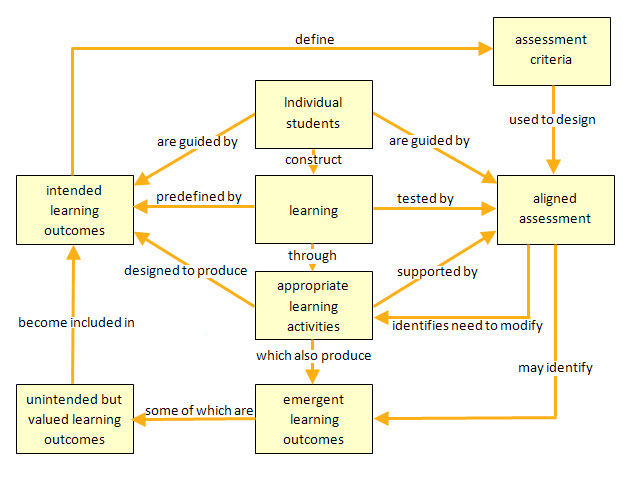
\includegraphics[width=\columnwidth]{Houghton_constructive_alignment_1}
% 	\caption{Constructive alignment model presented by Houghton in~\cite{Houghton:2004}}
% 	\label{fig:constructive_alignment}
% \end{figure}

The first stage of our research was to determine how Biggs' model of constructive alignment~\cite{Biggs:1996c}, and the details on using portfolio assessment suggested by Biggs and Tang in~\cite{Biggs:1997}, could be used to guide the creation of an introductory programming unit. Examining the practical advice from Biggs and Tang in~\cite{Biggs:2007}, which further elaborates on both his model of constructive alignment and portfolio assessment, a model of constructive alignment for introductory programming was defined. The model is presented in \fref{fig:process_overview}, which captures staff and student processes and the artefacts generated and exchanged throughout the learning process.

\begin{figure*}[t!]
	\centering
	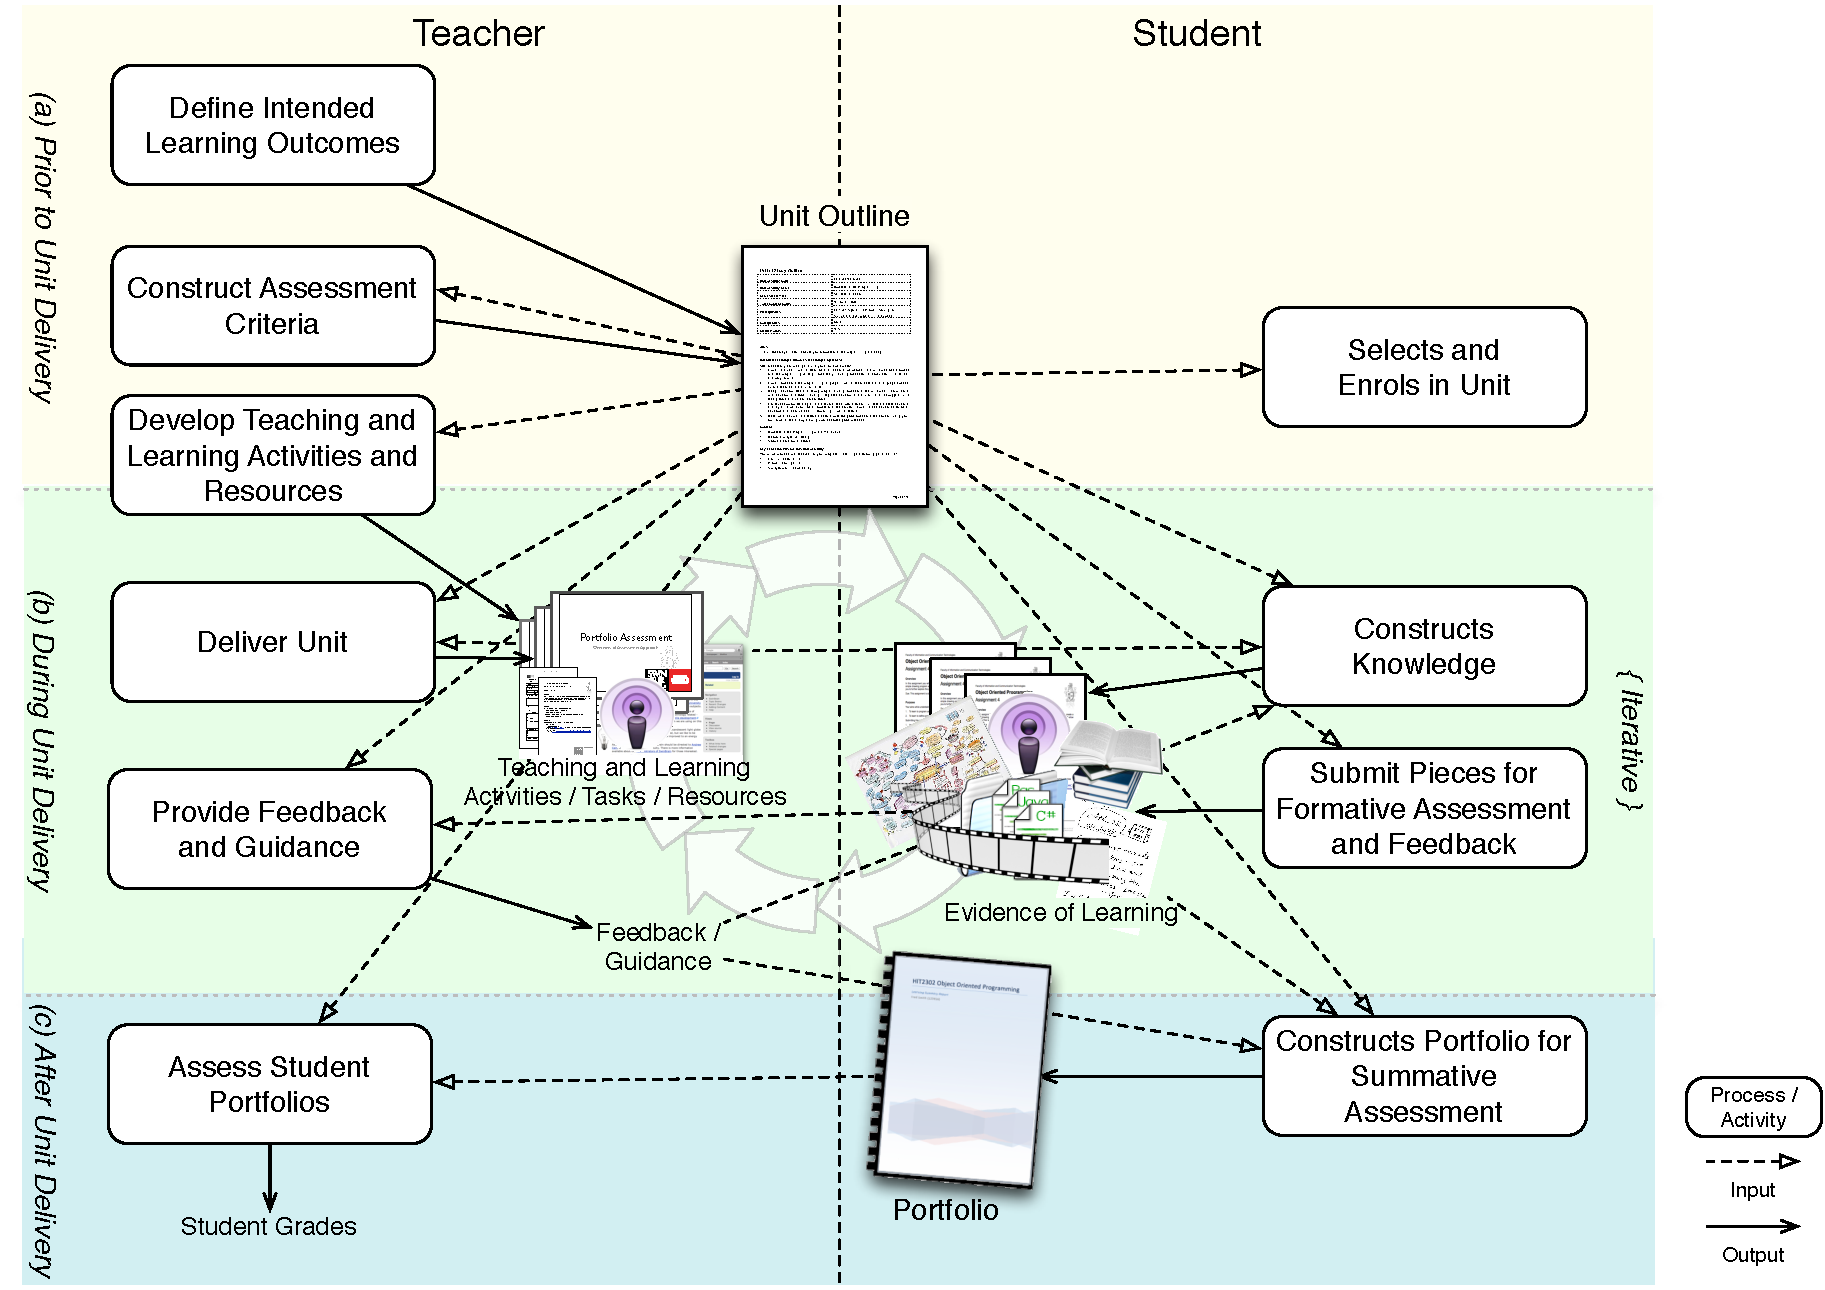
\includegraphics[width=6in]{ProcessOverview}
	\caption{An overview of teacher and students roles, and iterative delivery, in the constructive alignment model developed for introductory programming.}
	\label{fig:process_overview}
\end{figure*}

The model is divided into \emph{student} and \emph{teacher}\footnote{Teacher in this context encompasses all teaching staff related to the unit, though each stage may not involve all staff members.} processes, distributed throughout unit design and delivery. This is highlighted in \fref{fig:process_overview} by columns for the teacher and student processes, and three rows for the stages in which they occur. The stages identified are \emph{prior} to unit delivery, \emph{during} unit delivery, and \emph{post} unit delivery.

Prior to the unit delivery (a) the teaching staff \emph{define intended learning outcomes} and \emph{construct assessment criteria}, which together form the critical components of the unit outline. Such a document is a common practice, and forms the central focus for the unit. The unit outline is then used to inform and guide staff in the \emph{development of teaching and learning activities}. Unit outlines may also be used by students in evaluating units to select in their course.

During the teaching period (b), staff \emph{deliver the unit} using the developed teaching and learning activities. Ideally these activities help student's to \emph{construct knowledge}. As a result, students produce artefacts that demonstrate their depth of understanding, which may then be selected by the student and \emph{submitted for formative feedback}. This provides an opportunity for teaching staff to \emph{provide feedback and guidance}. The process of activities, knowledge construction, and formative feedback is designed to be an ongoing iterative process.

After the delivery of the unit (c) students \emph{construct and submit a portfolio for assessment}, which is then \emph{assessed by} the teaching staff against the intended learning outcomes and assessment criteria prepared prior to the unit's delivery.

The central role of intended learning outcomes and assessment criteria is to, as Biggs elegantly phrased it, ``entrap'' students ``in this web of consistency, optimising the likelihood that they will engage the appropriate learning activities.''~\cite{Biggs:1999}

While each of the processes described is important, some are of more interest than others when defining a constructively aligned approach. Of specific interest is the definition of the intended learning outcomes, the setting of the assessment criteria, the use of formative feedback during delivery, and the assessment of the portfolio.

\section{Model Process Details} % (fold)
\label{sec:process_details}

Here we outline the different processes of the model presented, with supportive examples from an initial implementation. The model was applied to a second level programming unit that focused on object oriented programming. Students are assumed to have been previously introduced to procedural programming, and as such were expected to have a working understanding of basic programming constructs (sequence, selection, repetition), as well as function and procedure declarations and parameter passing. 

The goals of the second programming unit were to introduce students to objects, object oriented principles, responsibility driven design, and to develop proficiency using an object oriented programming language. In this early example of the model's application, the unit was taken by 83 students and taught by a small team of staff. The model has been subsequently adapted and applied to other introductory programming units which are not dissimilar, though not discussed in this paper.

\subsection{Defining Intended Learning Outcomes} % (fold)
\label{sub:defining_intended_learning_outcomes}

When using constructive alignment, the intended learning outcomes are central to the assessment of the unit. With more \emph{traditional} forms of assessment, teaching staff take responsibility for aligning assessment to required outcomes. With portfolio assessment, teaching staff relinquish control of this aspect and the outcomes themselves take on a dual purpose: as a statement of what will be \emph{taught}, and what will be \emph{assessed}. Effectively the specified unit outcomes become the assessment, thereby taking advantage of the fact that ``assessment always drives the curriculum'' (Ramsden~\cite{Ramsden:1992}).  In this arrangement there is little opportunity for misalignment between the unit objectives and assessment, but a greater importance on the exact nature of the intended learning outcomes. This critical role of the intended learning outcomes means that they are instrumental in the success of the unit. 

For an introductory programming unit it is important to design the intended learning outcomes so that, as a group, they cover the required programming competencies as well as the associated conceptual knowledge. As the outcomes drive the entire process -- including both student and teacher processes -- it is important they are expressed clearly and simply so as to be understood by all involved.

A variety of sources serve as inputs into this process, though these are not shown in \fref{fig:process_overview}. In preparing learning outcomes, Thota and Whitfield propose inputs related to pedagogic theory (constructivism and phenomenography) as well as student factors such as approach to learning, learning styles, and prior knowledge. Armarego~\cite{Armarego:2009} highlights the needs for input related to industry requirements and domain characteristics, such as the Computer Science and Software Engineering Curriculum from professional standards bodies (see~\cite{Lethbridge:2006} and~\cite{Cassel:2008}), and associated Bodies of Knowledge (see~\cite{Abran:2001}).

We developed the following principles which can be used to guide the formation of the intended learning outcomes for portfolio assessed programming units:
\begin{itemize}
  \item Express outcomes using verbs at an appropriate level of understanding with reference to the SOLO taxonomy. (See~\cite{Biggs:2007} and~\cite{Biggs:1982}.)
  \item Cover both the required \emph{conceptual knowledge}, and \emph{programming competencies}.
  \item Use \emph{simple terms} (where possible) to communicate outcomes, ensuring they are understood by all students undertaking the unit.
  \item The number of outcomes should be \emph{minimal}, ideally between four and six (\emph{cf.}~\cite{Biggs:2007} and~\cite{Gardner:1994}). This is to help ensure that each outcome covers a meaningful body of knowledge to a sufficient depth.
  \item Outcomes need to be \emph{general} to facilitate assessment of diverse portfolios, and \emph{sufficient} to ensure that differing degrees of proficiency and understanding can be assessed.
  \item There needs to be \emph{flexibility} to enable students to choose a range of means when addressing outcomes.
\end{itemize}

In the example implementation presented in this work, the learning objectives had been predefined, as required by the outside influence of accreditation processes, but were expressed using appropriate action verbs. \tref{tbl:example_intended_learning_outcomes} lists the outcomes from the example unit delivered using this model.

\begin{table*}[!t]
  \footnotesize
% increase table row spacing, adjust to taste
\renewcommand{\arraystretch}{1.3}
% if using array.sty, it might be a good idea to tweak the value of
% \extrarowheight as needed to properly center the text within the cells
\caption{Example intended learning outcomes}
\label{tbl:example_intended_learning_outcomes}
\centering
% Some packages, such as MDW tools, offer better commands for making tables
% than the plain LaTeX2e tabular which is used here.
\begin{tabular}{|l p{6.25in}|}
\hline
1) & Explain the use, implementation of, and relationships between, the principles of the object oriented programming paradigm specifically including abstraction, encapsulation, inheritance, and polymorphism.
\\
\hline
2) & Explain object oriented programming language implementation details and language specific culture, features, and environments.
\\
\hline
3) & Design, develop, test, and debug programs using object oriented principles in conjuncture with development tools including integrated development environments, debuggers, unit testing tools, and version control tools. \\
\hline
4) & Construct appropriate diagrams and textual descriptions to communicate the static structure and dynamic behaviour of an object oriented solution, explain these structures to other developers, and convert them into working implementations.\\
\hline
5) & Describe and explain the factors that contribute to a good object oriented solution, using your own experiences and by drawing upon accepted good practices. \\
\hline
\end{tabular}
\end{table*}

% subsection defining_intended_learning_outcomes (end)






\subsection{Constructing Assessment Criteria} % (fold)
\label{sub:constructing_assessment_criteria}

Alongside the development of the intended learning outcomes is the definition of the assessment criteria. These criteria are used to assess student portfolios, but also guide the teaching and learning activities. Providing assessment criteria in the unit outline creates a simplified learning contract~\cite{Stephenson:1993}, in which students know ``up front'' what is required to achieve the different grade results.

To provide a holistic judgement, the portfolio assessment is \emph{criterion-referenced} as suggested by Biggs and Tang in~\cite{Biggs:1997}. The assessment criteria development process takes input from the intended learning outcomes, along with guidelines for portfolio assessment~\cite{Biggs:2007} and levels of achievement from the SOLO taxonomy~\cite{Biggs:1982}. The resulting criteria are also placed in the unit outline.

There is some contention regarding the specification of assessment criteria for assessing portfolios. For example, some consider that by overly specifying criteria students are limited in what can be included (see~\cite{Driessen:2005,Tigelaar:2007}). However, it was thought by the staff involved in this work that students in introductory programming units require specific guidance, a position supported by Thorpe~\cite{Thorpe:2000}, who suggests that students find it difficult to reflect on what they have learnt. Thorpe also noted that this process is made easier for students if they apply criteria defined by teaching staff. 

The following principles were used to guide the definition and communication of the assessment criteria:

\begin{itemize}
  \item \emph{Outline} what is required to achieve the different levels of understanding for each of the intended learning outcomes.
  \item Communicate assessment criteria using \emph{simple terms} (as suggested for the outcomes).
  \item Higher grades should require evidence of \emph{deeper learning}, while specifically avoiding an excessive volume of work.
  \item Clearly \emph{map assessment criteria} to grade outcomes, ensuring students and staff have a shared understanding of how a portfolio relates to final grades.
\end{itemize}

\begin{table*}[!t]
  \footnotesize
% increase table row spacing, adjust to taste
\renewcommand{\arraystretch}{1.3}
% if using array.sty, it might be a good idea to tweak the value of
% \extrarowheight as needed to properly center the text within the cells
\caption{Example Assessment Criteria related to the intended learning outcome 2 from Table~\ref{tbl:example_intended_learning_outcomes}}
\label{tbl:example_assessment_criteria}
\centering
% Some packages, such as MDW tools, offer better commands for making tables
% than the plain LaTeX2e tabular which is used here.
\begin{tabular}{|p{1.5in}|p{1.5in}|p{1.5in}|p{1.5in}|}
\hline
\textbf{Marginal} & \textbf{Adequate} & \textbf{Good} & \textbf{Excellent} \\
\hline
Evidence shows a minimally acceptable understanding of the language chosen and the ability to use the language to implement object oriented programs. 
&
There is evidence of adequate understanding of the language chosen and the ability to use it to implement object oriented programs.

Programs illustrate appropriate use of language features.

Programs illustrate a correct use of the language’s tools, and programming standards.
&
	Illustrates a good mastery of the language chosen, its culture, environment, and tools.

Programs illustrate appropriate use of language features, and evidence of considered selection of classes from the language’s class library.	
&
As in “good” but provides further depth through either:

\begin{itemize}
  \item Wider reading and the use of more advanced language features or classes, or
  \item Elegant application of the language to solve problems, or
  \item Other research or analysis related to programming languages.
\end{itemize}
\\
\hline
\end{tabular}
\end{table*}

\begin{table*}[!t]
  \footnotesize
% increase table row spacing, adjust to taste
\renewcommand{\arraystretch}{1.3}
% if using array.sty, it might be a good idea to tweak the value of
% \extrarowheight as needed to properly center the text within the cells
\caption{Example mapping from piece assessment, to final grades}
\label{tbl:example_mapping_to_grades}
\centering
% Some packages, such as MDW tools, offer better commands for making tables
% than the plain LaTeX2e tabular which is used here.
\begin{tabular}{|c|c|c|>{\centering\arraybackslash}m{0.375in}|>{\centering\arraybackslash}m{0.375in}|>{\centering\arraybackslash}m{0.375in}|>{\centering\arraybackslash}m{0.375in}|>{\centering\arraybackslash}m{0.375in}|>{\centering\arraybackslash}m{0.375in}|>{\centering\arraybackslash}m{0.375in}|>{\centering\arraybackslash}m{0.375in}|>{\centering\arraybackslash}m{0.375in}|}
\hline
\multicolumn{3}{|c|}{50 P} &
58 P & 62 P & 65 C & 75 D & 78 D & 82 D & 95 HD & 98 HD & 100 HD  \\
\hline
\multicolumn{3}{|p{1.5in}|}{All intended learning outcomes are addressed to at least a marginal level.

No outcomes are poor or missing.} &
\multicolumn{3}{|p{1.5in}|}{At least three of the intended learning outcomes are addressed to an adequate or higher level. 

Other outcomes are addressed at a marginal level.
} &
\multicolumn{3}{|p{1.5in}|}{At least two intended learning outcomes are at a good level or higher.

Other outcomes must be addressed to at least an adequate level.

No outcomes are marginal.
} &
\multicolumn{3}{|p{1.5in}|}{At least two of the intended learning outcomes are addressed to an excellent level.

All other outcomes are addressed to a good level.

No outcomes are less than good.
} \\

\hline
\end{tabular}
\end{table*}

In the example unit it was decided to grade each of the intended learning outcomes, and from this derive each student's grade result. \tref{tbl:example_assessment_criteria} shows the criteria for one of the intended learning outcomes from the example implementation. 

The assessment criteria were divided into four categories, following examples from~\cite{Biggs:2007}, representing \emph{marginal}, \emph{adequate}, \emph{good}, and \emph{excellent} evidence of the required learning. For each outcome the \emph{marginal} category was associated with minimally acceptable standards of achievement, \emph{adequate} with an understanding of core aspects, \emph{good} with an integrated understanding, and \emph{excellent} with higher degrees of originality or deeper levels of performance being demonstrated. These map to the SOLO taxonomy's multi-structural, and relational levels of achievement, with the \emph{excellent} category bordering on extended abstract.

Further criteria specified how the assessment of the individual learning outcomes formed the student's final grade. The criteria used is shown in \tref{tbl:example_mapping_to_grades}, and required that a number of the learning outcomes were met at the indicated level in order to achieve each grade. For example, a distinction required that at least two of the outcomes were at a \emph{good} level. This approach allowed students to focus on areas of the unit they were more interested in, while still ensuring that they demonstrated a good coverage for higher grades.

% subsection constructing_assessment_criteria (end)

\subsection{Iterative Delivery} % (fold)
\label{sub:iterative_delivery}

Constructive learning theories emphasise the active role of the learner in constructing knowledge. Biggs' model of constructive alignment takes a pragmatic view of constructivism, using the phrase ``It's what the student does that counts.''~\cite{Biggs:1996c} % , a statement that can be traced back to Tyler's quote, ``It is what he does that he learns, not what the teacher does''~\cite{Tyler:1969}.

Existing work on constructive approaches to teaching introductory programming provide some advice on designing and delivering student centred teaching and learning activities. Ben-Ari~\cite{BenAri:1998} discusses the need for students to construct appropriate models of the computer. Van Gorp and Grissom~\cite{VanGorp:2001} discuss collaborative and constructive environments with the use of code walkthroughs, writing code, debugging and other activities. Thramboulidis~\cite{Thramboulidis:2003a} presents a design first approach to object oriented programming. Wulf~\cite{Wulf:2005} discusses strategies such as moving content from lectures to online video presentations. Similarly the work of Thota and Whitfield~\cite{Thota:2010} also presents constructive approaches to teaching introductory programming.

\begin{figure}[t!]
	\centering
	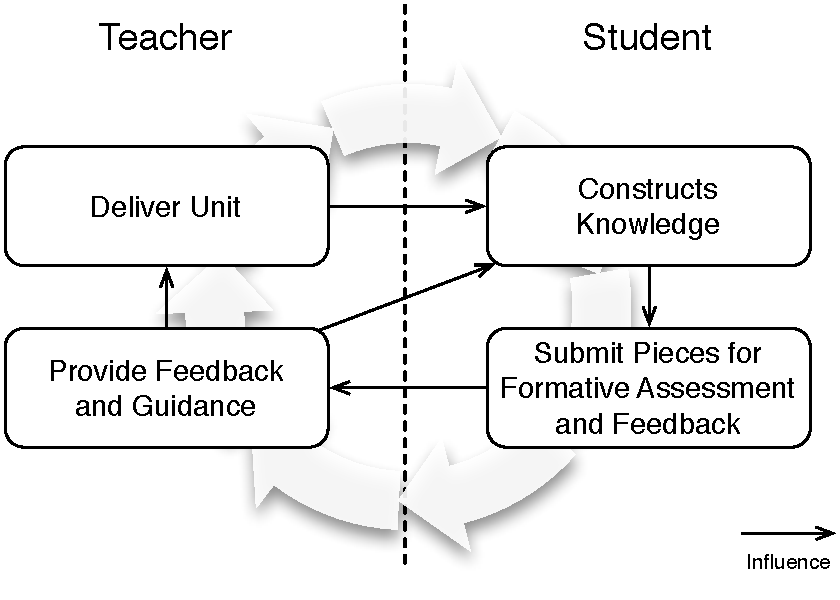
\includegraphics[width=2.5in]{DeliveryProcess}
	\caption{Iterative nature of the delivery process}
	\label{fig:delivery_overview}
\end{figure}

One critical aspect in our model is the iterative use of \emph{formative} feedback to help students construct appropriate knowledge, and to address misconceptions, as shown in \fref{fig:delivery_overview}. Teaching staff deliver teaching and learning activities to help students construct knowledge. These activities give students opportunities to create potential portfolio pieces that demonstrate their understanding. These pieces are submitted for feedback, that then inform future activities and provide students with advice they can use to help them address misconceptions, or otherwise improve their work.

The following principles were developed and used to guide the planning and delivery of teaching and learning activities:

\begin{itemize}
  \item Provide opportunities through activity design to actively engage students -- \emph{it is what the student does that counts}.  
  \item Relate all activities to the objectives, providing students with opportunities to create evidence for their portfolio.
  \item Use ungraded formative feedback to aid knowledge construction, with preference for small, frequent guidance.
\end{itemize}

In the example unit we avoided the use of traditional lecture style presentations, and included constructivist activities such as interactive presentations using audience response systems, role-plays, group design activities, and code walkthroughs. 

Students developed a number of programs based on constructive activities including a sort visualisation program (to introduce language constructs), a shape drawing program (to explore objects and inheritance), and a board game (to learn about object design and implementation for a larger problem).

% subsection the_role_of_formative_feedback (end)

\subsection{Constructing and Assessing Portfolios} % (fold)
\label{sub:assessing_the_portfolios}

The final phase of the process is the development and submission of portfolios by students, and assessment by staff. This process uses the outcomes and assessment criteria to determine what needs to be demonstrated and assessed. 

A number of papers discuss portfolio assessment for introductory programming units. Plimmer reports the successful use of portfolio assessment in an introductory programming unit in~\cite{Plimmer:2000}, where the portfolio contributed between 25\% and 60\% of the students' final grades. Programming portfolios were also discussed by Jones in~\cite{Jones:2010}, where students submitted a number of portfolio assignments during the semester. In both cases the portfolio was a collection of programs that were marked and contributed to a final grade.

Our proposed assessment model uses 100\% portfolio assessment. Formative feedback allows students to improve their understanding during delivery, without penalty for demonstrating their misunderstandings. The final portfolio then includes a student's best work, encouraging them to incorporate the feedback they receive. This is a highly considered position based on our own experience in prior units. Graded assessment during unit delivery encourages students to ``cover up'' their lack of knowledge or shallow understanding. Surely it must be the final outcomes that matter, not the rate of progress. With this in mind the common use of mid-term summative assessment is surprising.

% The use of an interview, or hurdle\footnote{In this case the hurdle test must be ``passed'' to pass the unit, but did not contribute to the final grade.} test, to help address plagiarism and increase confidence that the work in the portfolio is the students own work.

Based on our experience we suggest the following principles be used to guide the creation and assessment activities of portfolios:

\begin{itemize}
  \item Encourage unique, diverse, concise, and strongly aligned evidence.
  \item Motivate students to include evidence of learning from formative experience.
  \item Accurately and consistently follow the terms of the assessment criteria, as this is the \emph{contract} the students work towards.
  \item Require students to reflect on their learning, and the evidence in their portfolio, with respect to the intended learning outcomes of the unit and the assessment criteria.
  \item Use an interview, or hurdle\footnote{In this case the hurdle test must be ``passed'' to pass the unit, but did not contribute to the final grade.} test, to check minimal pass criteria in an invigilated manner. Where tests are used they need only distinguish between pass and fail, and do not need to address higher grades. 
\end{itemize}

Portfolios in the example unit were required to include a \emph{reflective report}, a \emph{hurdle test}, and additional pieces to demonstrate coverage of the learning outcomes. Students were encouraged to incorporate feedback they received during the delivery, and to include a range of pieces such as programs, reports, and concept maps. The hurdle test covered all basic content, and students had to demonstrate a good understanding of the principles covered in the unit, as well as sufficient programming proficiency. Where students failed the hurdle they were permitted to re-sit an equivalent test once.

% subsection assessing_the_portfolios (end)

% section process_details (end)

% subsection design_assessment_criteria (end)

% section design (end)

% section model (end)


\section{Discussion and Conclusion}

This work presents a model for applying constructive alignment with portfolio assessment for teaching introductory programming, along with principles to help guide the development and delivery of such units. The model and principles presented have been applied to the delivery of a number of introductory programming units, with positive feedback from students and staff. The initial implementation demonstrated the potential of the approach, with the model appearing to be worth further investigation, but the delivery requiring some adjustments. 

Students responded positively to the unit delivery as evidenced by the results in the university's student feedback on teaching survey. An additional survey was conducted to collect details on students approaches to learning, and their perceptions of the portfolio assessment. Only 16 students completed the survey with all comments being positive, as a quote from one student shows: 

\begin{quote}
  ``The portfolio was a great exercise, it stimulated me to do independent research and think about what I had learnt''   
\end{quote}

There were some challenges for staff related to a perceived \emph{loss of control}, \emph{via} vexation, with less motivated students not making the most of the formative opportunities. The unit had a lower than desired submission rate, with 64 portfolios being submitted from the initial enrolment of 83 students. Students achieved grades that indicate that the learning activities aligned with the outcomes, and interestingly resulted in an even distribution across the grade spectrum.

Future publications will examine the implementation of this model more fully; looking in more detail at the portfolios submitted, student approaches to learning, and possible adjustments to the model and principles in light of this analysis.


% chapter approaching_constructive_alignment_with_portfolio_assessment (end)